O meu plano de desenvolvimento pessoal, passa por obter mais formação e apreender com pessoas com mais experiência em diversas áreas, que é exatamente o que estou a fazer frequentando o curso de Engenharia Eletrotécnica e de Computadores no \textcolor{gray}{I.S.E.P}.\\
Esta disciplina em particular é uma forma de poder enriquecer minhas competências e metodologias de Gestão, e as restantes matérias abordadas que compõem o \textcolor{blue}{Comportamento Organizacional}.\\
\begin{minipage}{10.3cm}
\begin{figure}[H]
	%\flushleft
	\begin{minipage}{\linewidth}
		\flushleft
		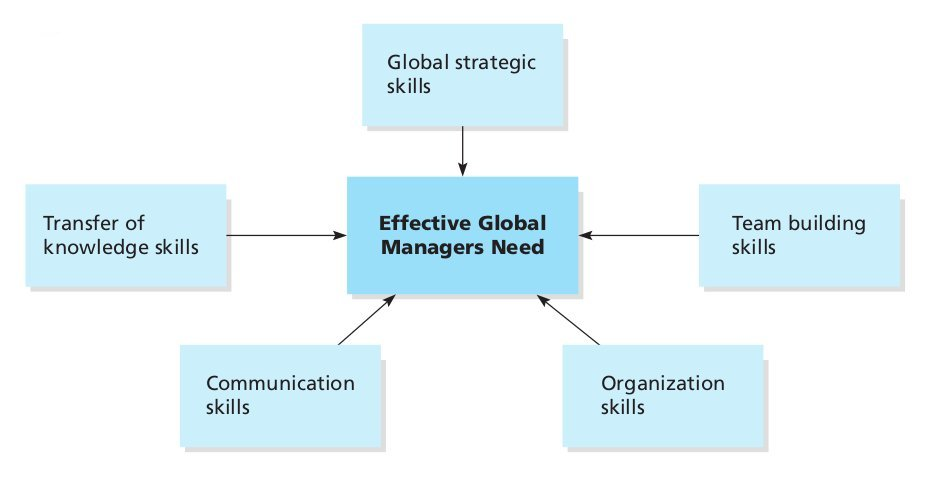
\includegraphics[scale=0.3]{"./image/Skills/Managerial Skills for the Global Marketplace.jpg"}
	\end{minipage}
	\caption{Competências de Gestão. \cite{book_6}}
\end{figure}
\end{minipage}
\begin{minipage}{12cm}
	\textbf{Metodologias da gestão}: \cite{book_9}\\
	\\
	\begin{minipage}{3.1cm}
		Instrumental
		\begin{enumerate}
			\setlength\itemsep{-0.3em}
			\item Planear
			\item Organizar
			\item Controlar\\
		\end{enumerate}
	\end{minipage}
	\begin{minipage}{5cm}
		Comportamental
		\begin{enumerate}
			\setlength\itemsep{-0.3em}
			\item Liderança
			\item Comunicação
			\item Motivação
			\item Tomada de decisão
		\end{enumerate}
	\end{minipage}
\end{minipage}





\begin{comment}
a) Realizar um diagnóstico de competências pessoais;\\
b) Definir objetivos de carreira;\\
c) Definir as competências que considere que no futuro lhe permitirão atingir os referidos objetivos;\\
d) Definir um plano de desenvolvimento para as competências anteriormente selecionadas.\\
Eliminate waste, reduce errors and improve.
\end{comment}